% BU ECE template for MS thesis and PhD dissertation.
%
%==========================================================================%
% MAIN PREAMBLE 
%==========================================================================%
\documentclass[12pt]{report}          % Single-sided printing for the library
%\documentclass[12pt,twoside]{report} % Double-sided printing
\usepackage[intlimits]{amsmath}
\usepackage{amsfonts,amssymb}
\DeclareSymbolFontAlphabet{\mathbb}{AMSb}
%\usepackage{natbib}
\usepackage{apalike}
\usepackage{float,subfigure}
\usepackage[bf]{caption}       
\setcaptionmargin{0.5in}
\usepackage{fancyheadings,fancybox,ifthen}
\usepackage{bu_ece_thesis}
\usepackage{url}
\usepackage{lscape,afterpage}
\usepackage{xspace}
\usepackage{color}
\usepackage{pdfpages}
%==========================================================================%
%%% graphicx and pdf creation
\usepackage{graphicx}
\definecolor{gray}{RGB}{102,102,102}
%\usepackage{psfrag}
%\DeclareGraphicsExtensions{.eps}   % extension for included graphics
%\usepackage{thumbpdf}              % thumbnails for ps2pdf
\usepackage[                       % hyper-references for ps2pdf
colorlinks=true,
linkcolor=black,
citecolor=gray,
bookmarks=true,%                   % generate bookmarks ...
bookmarksnumbered=true,%           % ... with numbers
%hypertexnames=false,%              % needed for correct links to figures !!!
%breaklinks=true,%                  % breaks lines, but links are very small
linkbordercolor={0 0 0},%          % blue frames around links
%pdfborder={0 0 112.0}				% border-width of frames 
]{hyperref}%  
%                                   % will be multiplied with 0.009 by ps2pdf
 \hypersetup{
  pdfauthor   = {Graham Voysey <gvoysey@bu.edu>},
  pdftitle    = {gvoysey-thesis.pdf},
  pdfsubject  = {Master's thesis},
  pdfkeywords = {biomedical engineering, hearing},
  pdfcreator  = {LaTeX/hyperref},
  pdfproducer = {LaTeX/P}
 }
%==========================================================================%
% customized commands can be placed here
%\newcommand{\figref}[1]{Figure~\ref{#1}}
%\newcommand{\chapref}[1]{Chapter~\ref{#1}}
%\newcommand{\latex}{\LaTeX\xspace}
%==========================================================================%

%==========================================================================%
% BEGIN
%==========================================================================%
\begin{document}

% The preliminary pages
% This file contains all the necessary setup and commands to create
% the preliminary pages according to the buthesis.sty option.

\title{Improved Brainstem Modeling to Characterize the Effect of Low Spontaneous Rate Fiber Loss on Auditory Neuropathy}

\author{Graham Voysey}

% Type of document prepared for this degree:
%   1 = Master of Science thesis,
%   2 = Doctor of Philisophy dissertation.
%   3 = Master of Science thesis and Doctor of Philisophy dissertation.
\degree=1

\prevdegrees{B.S., Boston University, 2006}

\department{Department of Biomedical Engineering}

% Degree year is the year the diploma is expected, and defense year is
% the year the dissertation is written up and defended. Often, these
% will be the same, except for January graduation, when your defense
% will be in the fall of year X, and your graduation will be in
% January of year X+1
\defenseyear{2016}
\degreeyear{2016}

% For each reader, specify appropriate label {First, second, third},
% then name, then title. Warning: If you have more than five readers
% you are out of luck, because it will overflow to a new page.
% Sometimes you may wish to put part of the title in with the name
\reader{First}{H. Steven Colburn, PhD}{Professor of Biomedical Engineering}
\reader{Second}{Barbara Shinn-Cunningham, PhD}{Professor of Biomedical Engineering}
\reader{Third}{Allyn E. Hubbard, PhD}{Professor of Electrical Engineering}

% The Major Professor is the same as the first reader, but must be
% specified again for the abstract page
\majorprof{H. Steven Colburn, PhD}{\mbox{Department of Biomedical Engineering}}

%                       PRELIMINARY PAGES
% According to the BU guide the preliminary pages consist of:
% title, copyright (optional), approval,  acknowledgments (opt.),
% abstract, preface (opt.), Table of contents, List of tables (if
% any), List of illustrations (if any). The \tableofcontents,
% \listoffigures, and \listoftables commands can be used in the
% appropriate places. For other things like preface, do it manually
% with something like \newpage\section*{Preface}.

% This is an additional page (do not hand it in at the library) to print
% boxed-in title, author and degree statement so that they are visible through
% the opening in BU covers used for reports. This makes a nicely bound copy.
%\buecethesistitleboxpage

% Make the titlepage based on the above information.  If you need
% something special and can't use the standard form, you can specify
% the exact text of the titlepage yourself.  Put it in a titlepage
% environment and leave blank lines where you want vertical space.
% The spaces will be adjusted to fill the entire page.
\maketitle
\cleardoublepage

% The copyright page is blank except for the notice at the bottom. You
% must provide your name in capitals.
\copyrightpage
\cleardoublepage

% Now include the approval page based on the readers information
\approvalpage
\cleardoublepage

% Here goes your favorite quote.
\newpage
\thispagestyle{empty}
% -*- root: ../gvoysey-thesis.tex -*-
\phantom{.}
\vspace{4in}

\begin{singlespace}
\begin{quote}
  We've heard a lot of models\ldots{}and heard suggested that we should take things out of our models to figure out what's important.  But in some sense, when I look at the diversity of models that have been presented so far---each of us leave out things.  So maybe in some sense we've got a start towards that approach.\\  
  
  So I can ask this question two ways, but let me ask it this way: \emph{What should we leave in?} What's the bare minimum we should leave in as we try to understand what's important about the function of the cochlea?
    % \textit{Facilis descensus Averni;}\\
  % \textit{Noctes atque dies patet atri janua Ditis;}\\*
  % \textit{Sed revocare gradum, superasque evadere ad auras,}\\
  % \textit{Hoc opus, hic labor est.}\hfill{Virgil (from Don's thesis!)}
  \vspace{2.5em}
  \begin{flushright}
  \textit{David C. Mountain\\Mechanics of Hearing (Attica, Greece 2014)}
  \end{flushright}
\end{quote}
\end{singlespace}
  

% \vspace{0.7in}
%
% \noindent
% [The descent to Avernus is easy; the gate of Pluto stands open night
% and day; but to retrace one's steps and return to the upper air, that
% is the toil, that the difficulty.]

\cleardoublepage

% The acknowledgment page should go here. Use something like
% \newpage\section*{Acknowledgments} followed by your text.
\newpage
\section*{\centerline{Acknowledgments}}
I would like to thank Jonathan Polimeni for cleaning up all these old
LaTeX style files and templates so that I didn't have to use Word to
write up this document. Also, I would like to thank all the CV/CNS lab
graduates for their contributions and tweaks to this organizational
scheme over the years (after many dissapointing interactions with
Martha Wellman).

This brings me to thank Martha Wellman of CAS and Brendon McDermot of
Mugar library who together uphold the stylistic and aesthetic
conventions that have been implemented in this LaTeX manuscript. Also
Sister Mary Virginia, the Thesis/dissertation coordinator of Mugar
Library, deserves some thanks as well.

Finally, I would like to thank Stephen Gildea, for the MIT sytle file
off which this current version is based, and Paolo Gaudiano for
porting the MIT style to one compatible for BU.

\cleardoublepage

% The abstractpage environment sets up everything on the page except
% the text itself.  The title and other header material are put at the
% top of the page, and the supervisors are listed at the bottom.  A
% new page is begun both before and after.  Of course, an abstract may
% be more than one page itself.  If you need more control over the
% format of the page, you can use the abstract environment, which puts
% the word "Abstract" at the beginning and single spaces its text.

\begin{abstractpage}
% ABSTRACT
My research is related to exploring the convergence of a recently discovered mechanism of hearing loss that is not detected in normal hearing tests called auditory neuropathy and the subjective phenomenon of tinnitus, or persistent ringing in the ears.   I have assembled a collection of models into a fuller simulation of this behavior, that helps to predict the likelihood and manner of maladaptive neuroplasticity in the brain that results from auditory neuropathy and may reflect a tinnitus state in humans. 
\end{abstractpage}
\cleardoublepage

% Now you can include a preface. Again, use something like
% \newpage\section*{Preface} followed by your text

% Table of contents comes after preface
\tableofcontents
\cleardoublepage

% If you have tables, uncomment the following line
%\listoftables
%\cleardoublepage

% If you have figures, uncomment the following line
\newpage
\listoffigures
\cleardoublepage

% List of Abbrevs is NOT optional (Martha Wellman likes all abbrevs listed)
\chapter*{List of Abbreviations}
\begin{center}
  \begin{tabular}{lll}
    \hspace*{2em} & \hspace*{1in} & \hspace*{4.5in} \\
    %CAD  & \dotfill & Computer-Aided Design \\   
    
  \end{tabular}
\end{center}
\cleardoublepage

% END OF THE PRELIMINARY PAGES

\newpage
\endofprelim
        
\cleardoublepage

% -------------------------------------
% CHAPTER 1: INTRODUCTION
% -------------------------------------
% -*- root: ../gvoysey-thesis.tex -*-
\chapter{Introduction}
\label{chapter:Introduction}
\thispagestyle{myheadings}

\section{A brief history}
\label{sec:history}

Let's get started.

\cleardoublepage

% -------------------------------------
% CHAPTER 2: THE BODY OF THESIS
% -------------------------------------
\chapter{Body of my thesis}
\label{chapter:body}
\thispagestyle{myheadings}

% set this to the location of the figures for this chapter. it may
% also want to be ../Figures/2_Body/ or something. make sure that
% it has a trailing directory separator (i.e., '/')!
\graphicspath{{2_Body/Figures/}}

\section{Some results}
\label{sec:results}

Here's the important stuff, and example of using graphics.

\begin{figure}[htb]
  \begin{minipage}[t]{0.49\linewidth}\centering
    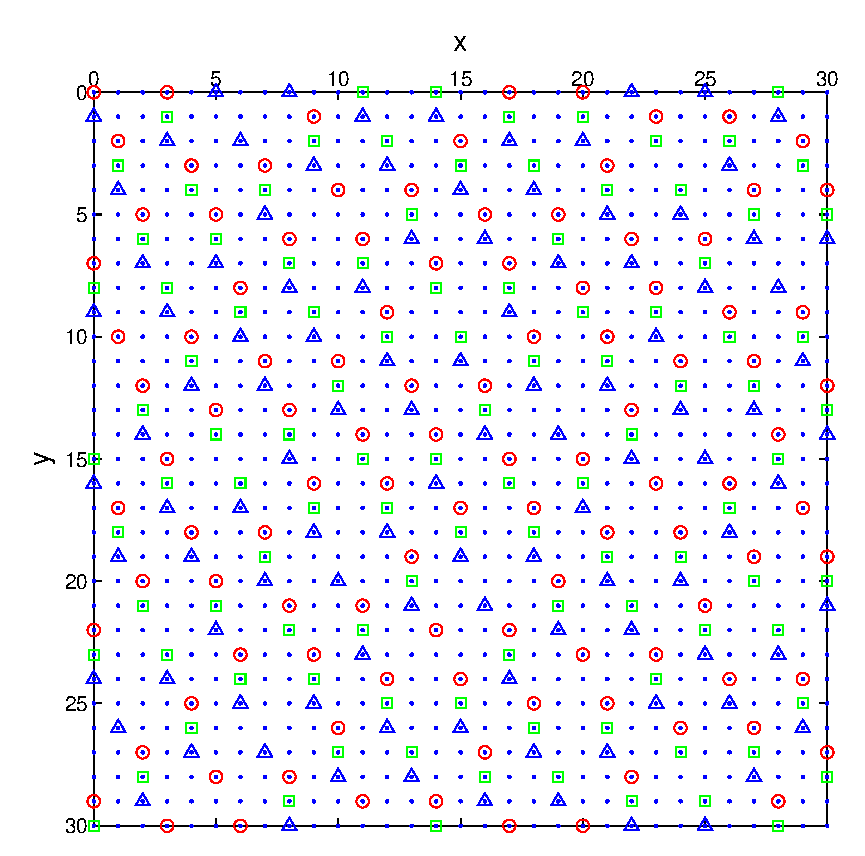
\includegraphics[width=7.7cm]{figure_sampling_view1.eps}
    \medskip
    \centerline{(a)}
  \end{minipage}\hfill
  \begin{minipage}[t]{0.49\linewidth}\centering
    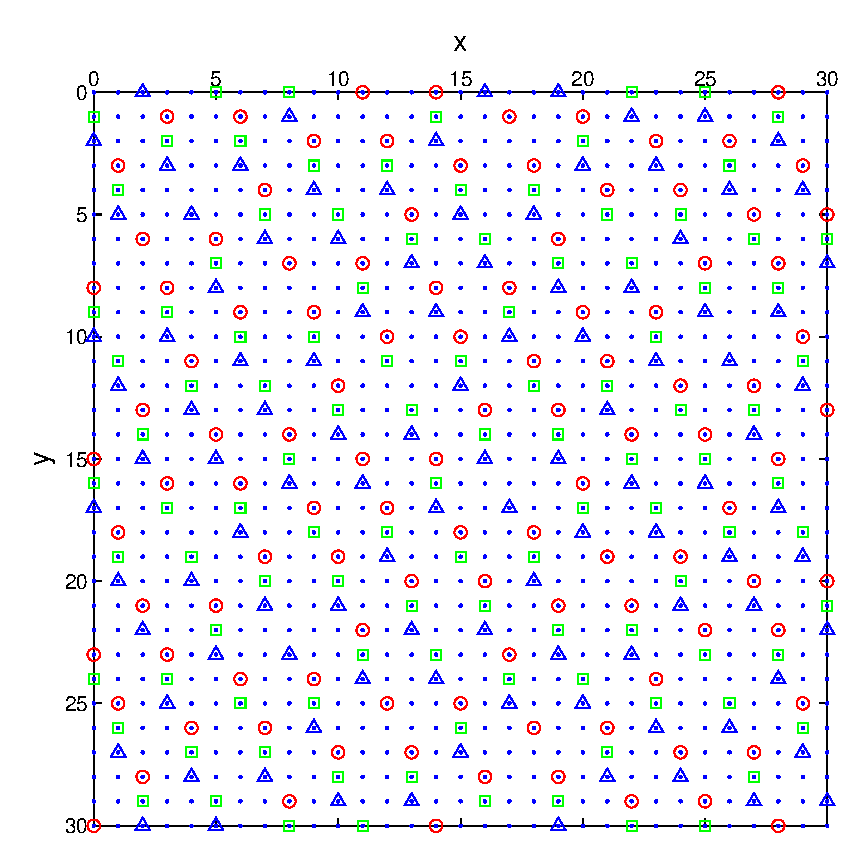
\includegraphics[width=7.7cm]{figure_sampling_view2.eps}
    \medskip
    \centerline{(b)}
  \end{minipage}
  \caption{Assignment of single-view intensities to RGB components: (a) view
    \#1; and (b) view \#2. }
  \label{fig:Sampling}
\end{figure}

And also how to use citations \cite{lamport1985:latex},\cite{Debr01}.

\cleardoublepage

% -------------------------------------
% CHAPTER 3: CONCLUSION
% -------------------------------------
\chapter{Conclusion}
\label{chapter:Conclusion}
\thispagestyle{myheadings}

% set this to the location of the figures for this chapter. it may
% also want to be ../Figures/2_Body/ or something. make sure that
% it has a trailing directory separator (i.e., '/')!
\graphicspath{{3_Conclusion/Figures/}}

\section{Pontifications}

Time to get philosophical and wordy.

\cleardoublepage

%==========================================================================%
% Bibliography
\newpage
\singlespace
\bibliographystyle{apalike}

% each subdirectory can have its own BiBTeX file
\bibliography{Remote}
\cleardoublepage

%==========================================================================%
% Curriculum Vitae
% TODO -- uncomment this one day and check this symlink so that it points to the correct version of the CV. 
%\includepdf[pages={ - }]{0_Prelim/gvoysey-cv.pdf}

%==========================================================================%
\end{document}
 